%2multibyte Version: 5.50.0.2960 CodePage: 1252

\documentclass[notes=show,handout]{beamer}
%%%%%%%%%%%%%%%%%%%%%%%%%%%%%%%%%%%%%%%%%%%%%%%%%%%%%%%%%%%%%%%%%%%%%%%%%%%%%%%%%%%%%%%%%%%%%%%%%%%%%%%%%%%%%%%%%%%%%%%%%%%%%%%%%%%%%%%%%%%%%%%%%%%%%%%%%%%%%%%%%%%%%%%%%%%%%%%%%%%%%%%%%%%%%%%%%%%%%%%%%%%%%%%%%%%%%%%%%%%%%%%%%%%%%%%%%%%%%%%%%%%%%%%%%%%%
\usepackage{amsfonts}
\usepackage{amsmath}
\usepackage{graphicx}
\usepackage{mathpazo}
\usepackage{hyperref}
\usepackage{multimedia}

\setcounter{MaxMatrixCols}{10}

\newenvironment{stepenumerate}{\begin{enumerate}[<+->]}{\end{enumerate}}
\newenvironment{stepitemize}{\begin{itemize}[<+->]}{\end{itemize} }
\newenvironment{stepenumeratewithalert}{\begin{enumerate}[<+-| alert@+>]}{\end{enumerate}}
\newenvironment{stepitemizewithalert}{\begin{itemize}[<+-| alert@+>]}{\end{itemize} }
\usetheme{Madrid}

\setcounter{MaxMatrixCols}{10}
\newtheorem{remark}{Remark}[section]
\newtheorem{proposition}{Proposition}[section]
\newtheorem{interpretation}{Interpretation}[section]
\newtheorem{goal}{Goal}[section]
\newtheorem{statement}{Statement}[section]
\newtheorem{aes}{Aim \& Scope}[section]
\newtheorem{exercise}{Exercise}[section]
\renewcommand{\Pr}{P}



\begin{document}



\title[S110015]{Probability I}
\subtitle{Lecture 9}
\author[La Vecchia]{Davide La Vecchia}
\date{Spring Semester 2020}
\maketitle

%TCIMACRO{\TeXButton{BeginFrame}{\begin{frame}}}%
%BeginExpansion
%\begin{frame}%
%%EndExpansion
%
%%\subsection{Jointly distributed discrete random variables}
%
%%%TCIMACRO{\TeXButton{BeginFrame}{\begin{frame}}}%
%%%BeginExpansion
%%\begin{frame}%
%%%EndExpansion
%%
%\frametitle{Jointly distributed discrete random variables}
%%
%\begin{example}
%\begin{stepitemize}
%\item Two production lines manufacture a certain type of item.
%
%\item Suppose that the capacity (on any given day) is 5 items for \emph{Line
%I }and 3 items for \emph{Line II}.
%
%\item Assume that the number of items actually produced by either production
%line is a random variable.
%
%\item Let $(X,Y)$ represent the 2-dimensional random variable yielding the
%number of items produced by \emph{Line I} and \emph{Line II}, respectively.
%
%\item The joint probability (mass) function is 
%$$
%\Pr(\{X=x \quad \text{and} \quad Y=y\})
%$$
%for all possible values $x$ and $y$
%\end{stepitemize}
%\end{example}
%\end{frame}%
%
%
%\begin{frame}
%\frametitle{Jointly distributed discrete random variables}
%\begin{example}[cont'd]
%\begin{tabular}{|cc||c|c|c|c|c|c||c|}
%\hline
%& $x$ & $0$ & $1$ & $2$ & $3$ & $4$ & $5$ & $\Pr \left\{ Y=y\right\} $ \\
%$y$ &  &  &  &  &  &  &  &  \\ \hline\hline
%$0$ &  & $0$ & $0.01$ & $0.03$ & $0.05$ & $0.07$ & $0.09$ & $0.25$ \\ \hline
%$1$ &  & $0.01$ & $0.02$ & $0.04$ & $0.05$ & $0.06$ & $0.08$ & $0.26$ \\
%\hline
%$2$ &  & $0.01$ & $0.03$ & $0.05$ & $0.05$ & $0.05$ & $0.06$ & $0.25$ \\
%\hline
%$3$ &  & $0.01$ & $0.02$ & $0.04$ & $0.06$ & $0.06$ & $0.05$ & $0.24$ \\
%\hline\hline
%$\Pr \left\{ X=x\right\} $ &  & $0.03$ & $0.08$ & $0.16$ & $0.21$ & $0.24$ &
%$0.28$ & $1$ \\ \hline
%\end{tabular}
%\end{example}
%\end{frame}%


\begin{frame}
\frametitle{Joint Probability Functions}

\begin{stepitemize}
\item Let $X$ and $Y$ be a pair of discrete random variables

\item Their  \textbf{joint probability mass function} (joint
PMF) expresses the probability that simultaneously $X$ takes on the specific
value $x$ and $Y$ takes on the specific value $y$.

\item It is denoted by 
\begin{equation*}
p_{X,Y}\left( x,y\right) =\Pr (\left\{ X=x\cap Y=y\right\})
\end{equation*}
thought of as a function of $x$ and $y$.

\item The joint PMF has two essential properties:

\begin{stepenumerate}
\item $p_{X,Y}\left( x,y\right) \geq 0$ for all possible pairs $\left(
x,y\right) $ (its value is always non-negative)

\item $\sum_{x}\sum_{y}\Pr ( \left\{ X=x\cap Y=y\right\}) =1$ (its sum over all
combinations of $x$ and $y$ values is equal to one)
\end{stepenumerate}
\end{stepitemize}

%TCIMACRO{\TeXButton{EndFrame}{\end{frame}}}%
%BeginExpansion
\end{frame}%

\begin{frame}%
\frametitle{Marginal probability (mass) functions}

\begin{definition}
The probability (mass) function of the \emph{discrete} random variable 
$X$ is called its marginal probability (mass) function. It is obtained by summing the joint probabilities relating to pairs $%
(X,Y)$ over all possible values of $Y$:%
\begin{equation*}
p_{X}(x)=\sum_{y}p_{X,Y}(x,y).
\end{equation*}

Similarly, the probability (mass) function of the \emph{discrete}
random variable $Y$ is called its marginal probability (mass) function. It is obtained by summing the joint probabilities relating to pairs $%
(X,Y)$ over\emph{\ }all possible values of $X$:%
\begin{equation*}
p_{Y}(y)=\sum_{x}p_{X,Y}(x,y).
\end{equation*}
\end{definition}
\end{frame}%


\begin{frame}%
%EndExpansion

\frametitle{First Example }

\begin{example}[caplets: this probability course is giving me headache]
\begin{stepitemize}
\item Two caplets are selected at random from a bottle containing three
aspirins, two sedatives and two placebo caplets. We are assuming that the caplets are well mixed and that each has an
equal chance of being selected.

\item Let $X$ and $Y$ denote, respectively, the numbers of aspirin caplets,
and the number of sedative caplets, included among the two caplets drawn
from the bottle.
%
%\item We want to find the probabilities associated with all possible values
%of $X$ and $Y$.
%
%\item All the possible pairs of $(X,Y)$ are $(0,0)$,$(1,0)$, $(0,1)$, $(1,1)$%
%, $(2,0)$, and $(0,2)$.
\end{stepitemize}
\end{example}

%TCIMACRO{\TeXButton{EndFrame}{\end{frame}}}%
%BeginExpansion
\end{frame}%


%\begin{frame}%
%%EndExpansion
%
%\frametitle{First Example}
%
%%\begin{example}[cont'd]
%\begin{stepitemize}
%\item To work out each of these probabilties, we use combinations.
%
%\begin{stepitemize}
%\item e.g., the outcome $(1,1)$ corresponds to choosing only one asprin
%caplet and only one sedative caplet.
%
%\begin{stepitemize}
%\item But that one asprin caplet could be any one of the three available in
%the jar,
%
%\item and that one sedative caplet could be either one of the two available
%in the jar.
%
%\item So the number of possible combinations that satisfy $\left( x,y\right)
%=(1,1)$ are%
%\begin{eqnarray*}
%\underset{\text{\# asprin}}{\underbrace{\left( 
%\begin{array}{c}
%3 \\ 
%1%
%\end{array}%
%\right) }}\times \underset{\text{\# sedative}}{\underbrace{\left( 
%\begin{array}{c}
%2 \\ 
%1%
%\end{array}%
%\right) }}\times \underset{\text{\# placebo}}{\underbrace{\left( 
%\begin{array}{c}
%2 \\ 
%0%
%\end{array}%
%\right) }} &=&\frac{3!}{1!2!}\times \frac{2!}{1!1!}\times \frac{2!}{2!0!} \\
%&=&3\times 2\times 1=6
%\end{eqnarray*}
%\end{stepitemize}
%
%\item We can work out the number of possible combinations for the remaining $%
%\left( x,y\right) $ pairs similarly.
%\end{stepitemize}
%\end{stepitemize}
%%\end{example}
%%TCIMACRO{\TeXButton{EndFrame}{\end{frame}}}%
%%BeginExpansion
%\end{frame}%
%%EndExpansion
%%
%%%%TCIMACRO{\TeXButton{BeginFrame}{\begin{frame}}}%
%%%BeginExpansion
%\begin{frame}%
%%EndExpansion
%
%\frametitle{First Example (Discrete)}
%
%The \emph{probability} can be tabulated as
%
%\begin{center}
%\begin{tabular}{|c||c||c||c|}
%\hline
%${\small (x,y)}$ & {\small event drawn} & {\small combinations} & $\Pr
%\left\{ \left( X,Y\right) =\left( x,y\right) \right\} $ \\ \hline\hline
%${\small (0,0)}$ & {\small 2 placebos} & ${\small 1}$ & ${\small 1/21}$ \\ 
%\hline
%${\small (1,0)}$ & {\small 1 asprin,1 placebo} & ${\small 6}$ & ${\small 6/21%
%}$ \\ \hline
%${\small (0,1)}$ & {\small 1 sedative, 1 placebo} & ${\small 4}$ & ${\small %
%4/21}$ \\ \hline
%${\small (1,1)}$ & {\small 1 asprin, 1 placebo} & ${\small 6}$ & ${\small %
%6/21}$ \\ \hline
%${\small (2,0)}$ & {\small 2 asprin} & ${\small 3}$ & ${\small 3/21}$ \\ 
%\hline
%${\small (0,2)}$ & {\small 2 sedatives} & ${\small 1}$ & ${\small 1/21}$ \\ 
%\hline\hline
%{\small Total} &  & ${\small 21}$ & ${\small 1}$ \\ \hline
%\end{tabular}
%\end{center}
%
%TCIMACRO{\TeXButton{EndFrame}{\end{frame}}}%
%BeginExpansion
%\end{frame}%
%%EndExpansion
%
%%TCIMACRO{\TeXButton{BeginFrame}{\begin{frame}}}%
%%BeginExpansion
\begin{frame}%
%EndExpansion

\frametitle{First Example}

\begin{example}[cont'd]
Tabulating the \underline{\emph{joint}} probabilities as follows, 
we can easily work out the \underline{\emph{marginal}}
probabilities

\begin{center}
$%
\begin{tabular}{|cc||c|c|c||c|}
\hline
& $x$ & $0$ & $1$ & $2$ & $\Pr \left\{ Y=y\right\} $ \\ 
$y$ &  &  &  &  &  \\ \hline\hline
$0$ &  & $1/21$ & $6/21$ & $3/21$ & $10/21$ \\ \hline
$1$ &  & $4/21$ & $6/21$ & $0$ & $10/21$ \\ \hline
$2$ &  & $1/21$ & $0$ & $0$ & $1/21$ \\ \hline\hline
$\Pr \left\{ X=x\right\} $ &  & $6/21$ & $12/21$ & $3/21$ & $1$ \\ \hline
\end{tabular}%
$
\end{center}
\end{example}
%\begin{stepitemize}
%\item Note that the expected value for $X$ and $Y$ are, respectively,
%
%\begin{stepitemize}
%\item $E\left( X\right) =0\times 6/21+1\times 12/21+2\times 3/21=18/21=6/7$
%
%\item $E\left( Y\right) =0\times 10/21+1\times 10/21+2\times 1/21=12/21=4/7$
%\end{stepitemize}
%\end{stepitemize}

%TCIMACRO{\TeXButton{EndFrame}{\end{frame}}}%
%BeginExpansion
\end{frame}%


\begin{frame}%
%EndExpansion

\frametitle{Empirical Example}

\begin{example}

\begin{stepitemize}
\item Two production lines manufacture a certain type of item.

\item Suppose that the capacity (on any given day) is 5 items for \emph{Line
I }and 3 items for \emph{Line II}.

\item Assume that the number of items actually produced by either production
line varies from one day to the next.

\item Let $(X,Y)$ represent the 2-dimensional random variable yielding the
number of items produced by \emph{Line I} and \emph{Line II}, respectively,
on any one day.

\item In practical applications of this type the joint probability (mass)
function $\Pr(\{X=x\cap Y=y\})$ is unknown more often than not!
\end{stepitemize}
\end{example}

%TCIMACRO{\TeXButton{EndFrame}{\end{frame}}}%
%BeginExpansion
\end{frame}%
%EndExpansion

%TCIMACRO{\TeXButton{BeginFrame}{\begin{frame}}}%
%BeginExpansion
\begin{frame}%
%EndExpansion

\frametitle{Empirical Example}

\begin{example}

\begin{stepitemize}
\item The joint probability (mass) function $\Pr(\{X=x\cap Y=y\})$ for all
possible values of $x$ and $y$ can be approximated however.

\item By the observing the long-run relative frequency with which different
numbers of items are actually produced by either production line.
\end{stepitemize}

\begin{tabular}{|cc||c|c|c|c|c|c||c|}
\hline
& $x$ & $0$ & $1$ & $2$ & $3$ & $4$ & $5$ & $\Pr \left\{ Y=y\right\} $ \\ 
$y$ &  &  &  &  &  &  &  &  \\ \hline\hline
$0$ &  & $0$ & $0.01$ & $0.03$ & $0.05$ & $0.07$ & $0.09$ & $0.25$ \\ \hline
$1$ &  & $0.01$ & $0.02$ & $0.04$ & $0.05$ & $0.06$ & $0.08$ & $0.26$ \\ 
\hline
$2$ &  & $0.01$ & $0.03$ & $0.05$ & $0.05$ & $0.05$ & $0.06$ & $0.25$ \\ 
\hline
$3$ &  & $0.01$ & $0.02$ & $0.04$ & $0.06$ & $0.06$ & $0.05$ & $0.24$ \\ 
\hline\hline
$\Pr \left\{ X=x\right\} $ &  & $0.03$ & $0.08$ & $0.16$ & $0.21$ & $0.24$ & 
$0.28$ & $1$ \\ \hline
\end{tabular}

\begin{stepitemize}

\item e.g. $\Pr(\{X=5\cap Y=0\})\approx 0.09=\frac{\#\{X=5\cap Y=0\}\text{days}%
}{\#\text{days}}$ 
\end{stepitemize}
\end{example}

%TCIMACRO{\TeXButton{EndFrame}{\end{frame}}}%
%BeginExpansion
\end{frame}%
%EndExpansion

%TCIMACRO{\TeXButton{BeginFrame}{\begin{frame}}}%
%BeginExpansion
\begin{frame}%
%EndExpansion

\frametitle{Conditional probability mass function}

Recall that the \emph{conditional} probability mass function of the \emph{discrete 
}random variable $Y$, \emph{given} that the random variable $X$ takes the
value $x$, is given by%
\begin{equation*}
p_{Y|X}\left( y|x\right) =\frac{\Pr \left\{ X=x\cap Y=y\right\} }{%
P_{X}\left( X=x\right) }
\end{equation*}

Note this is a probability mass function for $y,$ with $x$ viewed as
fixed. Similarly, 

\begin{definition}
The \emph{conditional} probability mass function of the 
\emph{discrete }random variable $X$, \emph{given} that the random variable $%
Y $ takes the value $y$, is given by%
\begin{equation*}
p_{X|Y}\left( x|y\right) =\frac{\Pr \left\{ X=x\cap Y=y\right\} }{%
P_{Y}\left( Y=y\right) }
\end{equation*}
\end{definition}

Note this is a probability mass function for $x,$ with $y$ viewed as
fixed.

%TCIMACRO{\TeXButton{EndFrame}{\end{frame}}}%
%BeginExpansion
\end{frame}%
%EndExpansion

%%TCIMACRO{\TeXButton{BeginFrame}{\begin{frame}}}%
%%BeginExpansion
%\begin{frame}%
%%EndExpansion
%
%\frametitle{Conditional density functions}
%
%\begin{stepitemize}
%\item The \emph{conditional} (probability) density function of the random
%variable $Y$, given that the \emph{continuous }random variable $X$ takes the
%value $x$, is given by%
%\begin{equation*}
%f_{Y|X}\left( y|x\right) =\frac{f_{X,Y}\left( x,y\right) }{f_{X}\left(
%x\right) }
%\end{equation*}
%
%\begin{stepitemize}
%\item for every value of $y.$ Note this is a pdf for $y$, with $x$ viewed as
%fixed.\ 
%\end{stepitemize}
%
%\item Similarly, the \emph{conditional} (probability) density function of
%the random variable $X$, given that the \emph{continuous }random variable $Y$
%takes the value $y$, is given by%
%\begin{equation*}
%f_{X|Y}\left( x|y\right) =\frac{f_{X,Y}\left( x,y\right) }{f_{Y}\left(
%y\right) }
%\end{equation*}
%
%\begin{stepitemize}
%\item for every value of $x$ \ Note this is a pdf for $x$, with $y$ viewed
%as fixed.
%\end{stepitemize}
%\end{stepitemize}
%
%%TCIMACRO{\TeXButton{EndFrame}{\end{frame}}}%
%%BeginExpansion
%\end{frame}%
%%EndExpansion
%
%%TCIMACRO{\TeXButton{BeginFrame}{\begin{frame}}}%
%%BeginExpansion
\begin{frame}%
%EndExpansion

\frametitle{Independence }

\begin{stepitemize}
\item Two random variables $X$ and $Y$ are \textbf{independent} if 
\begin{eqnarray*}
p_{X,Y}(x,y) &=&p_{X}(x)p_{Y}(y)\qquad \qquad \text{(discrete)} \\
%f_{X,Y}(x,y) &=&f_{X}(x)f_{Y}(y)\qquad \qquad \text{(continuous)}
\end{eqnarray*}

 for \emph{all} values of $x$ and $y.$

\item Note that independence also implies that 
\begin{eqnarray*}
p_{X|Y}(x|y) &=&p_{X}(x)\text{ and }p_{Y|X}(y|x)=p_{Y}(y)\qquad \text{%
(discrete)} \\
%f_{X|Y}(x|y) &=&f_{X}(x)\text{ and }f_{Y|X}(y|x)=f_{Y}(y)\qquad \text{%
%(continuous)}
\end{eqnarray*}

for \emph{all} values of $x$ and $y.$
\end{stepitemize}

%TCIMACRO{\TeXButton{EndFrame}{\end{frame}}}%
%BeginExpansion
\end{frame}


\begin{frame}
\frametitle{Expectations for Jointly Distributed Discrete RVs}
\begin{example}
\begin{figure}[ptb]\centering
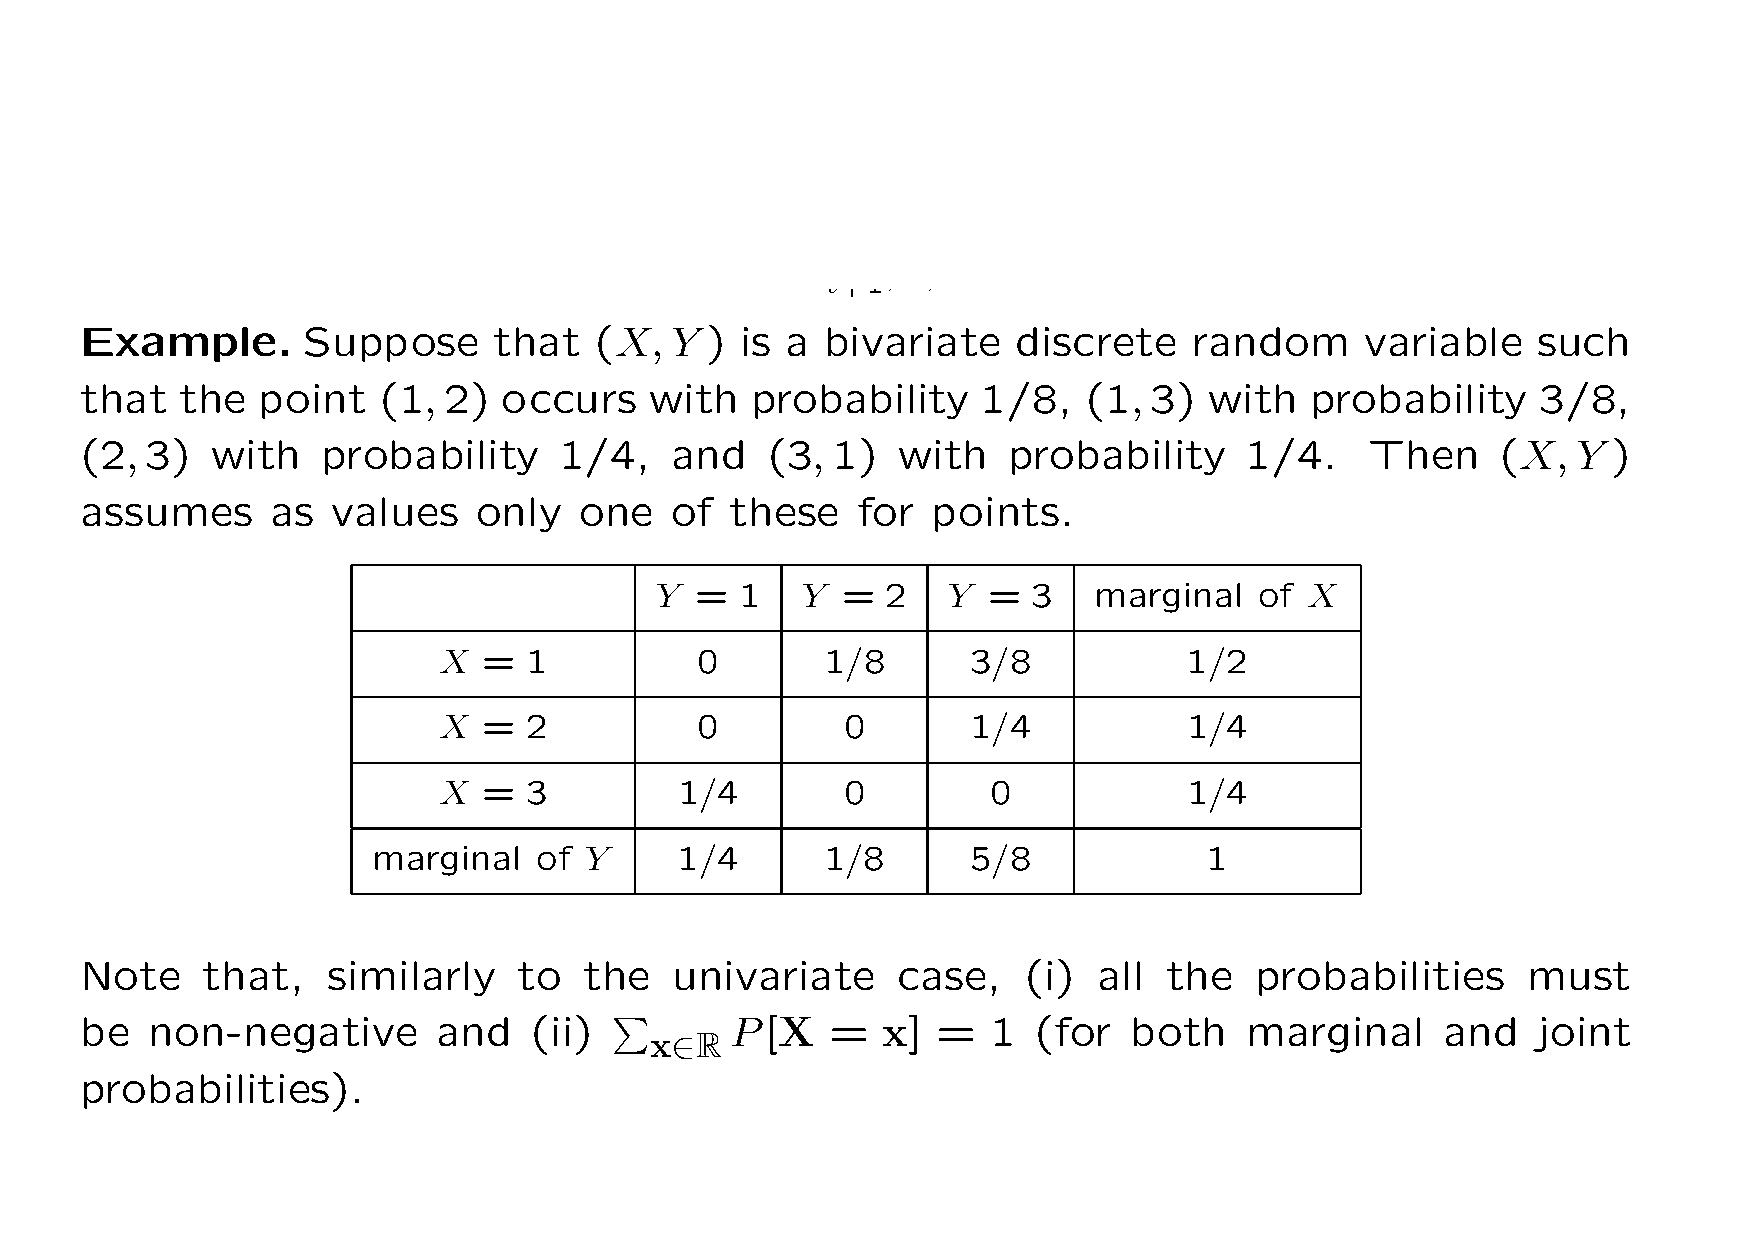
\includegraphics[width=0.95\textwidth,height=0.75\textheight]{ex_audrins.pdf}
\end{figure}
\end{example}
\end{frame}


\begin{frame}
\frametitle{Expectations for Jointly Distributed Discrete RVs}
\begin{example}
\begin{figure}[ptb]\centering
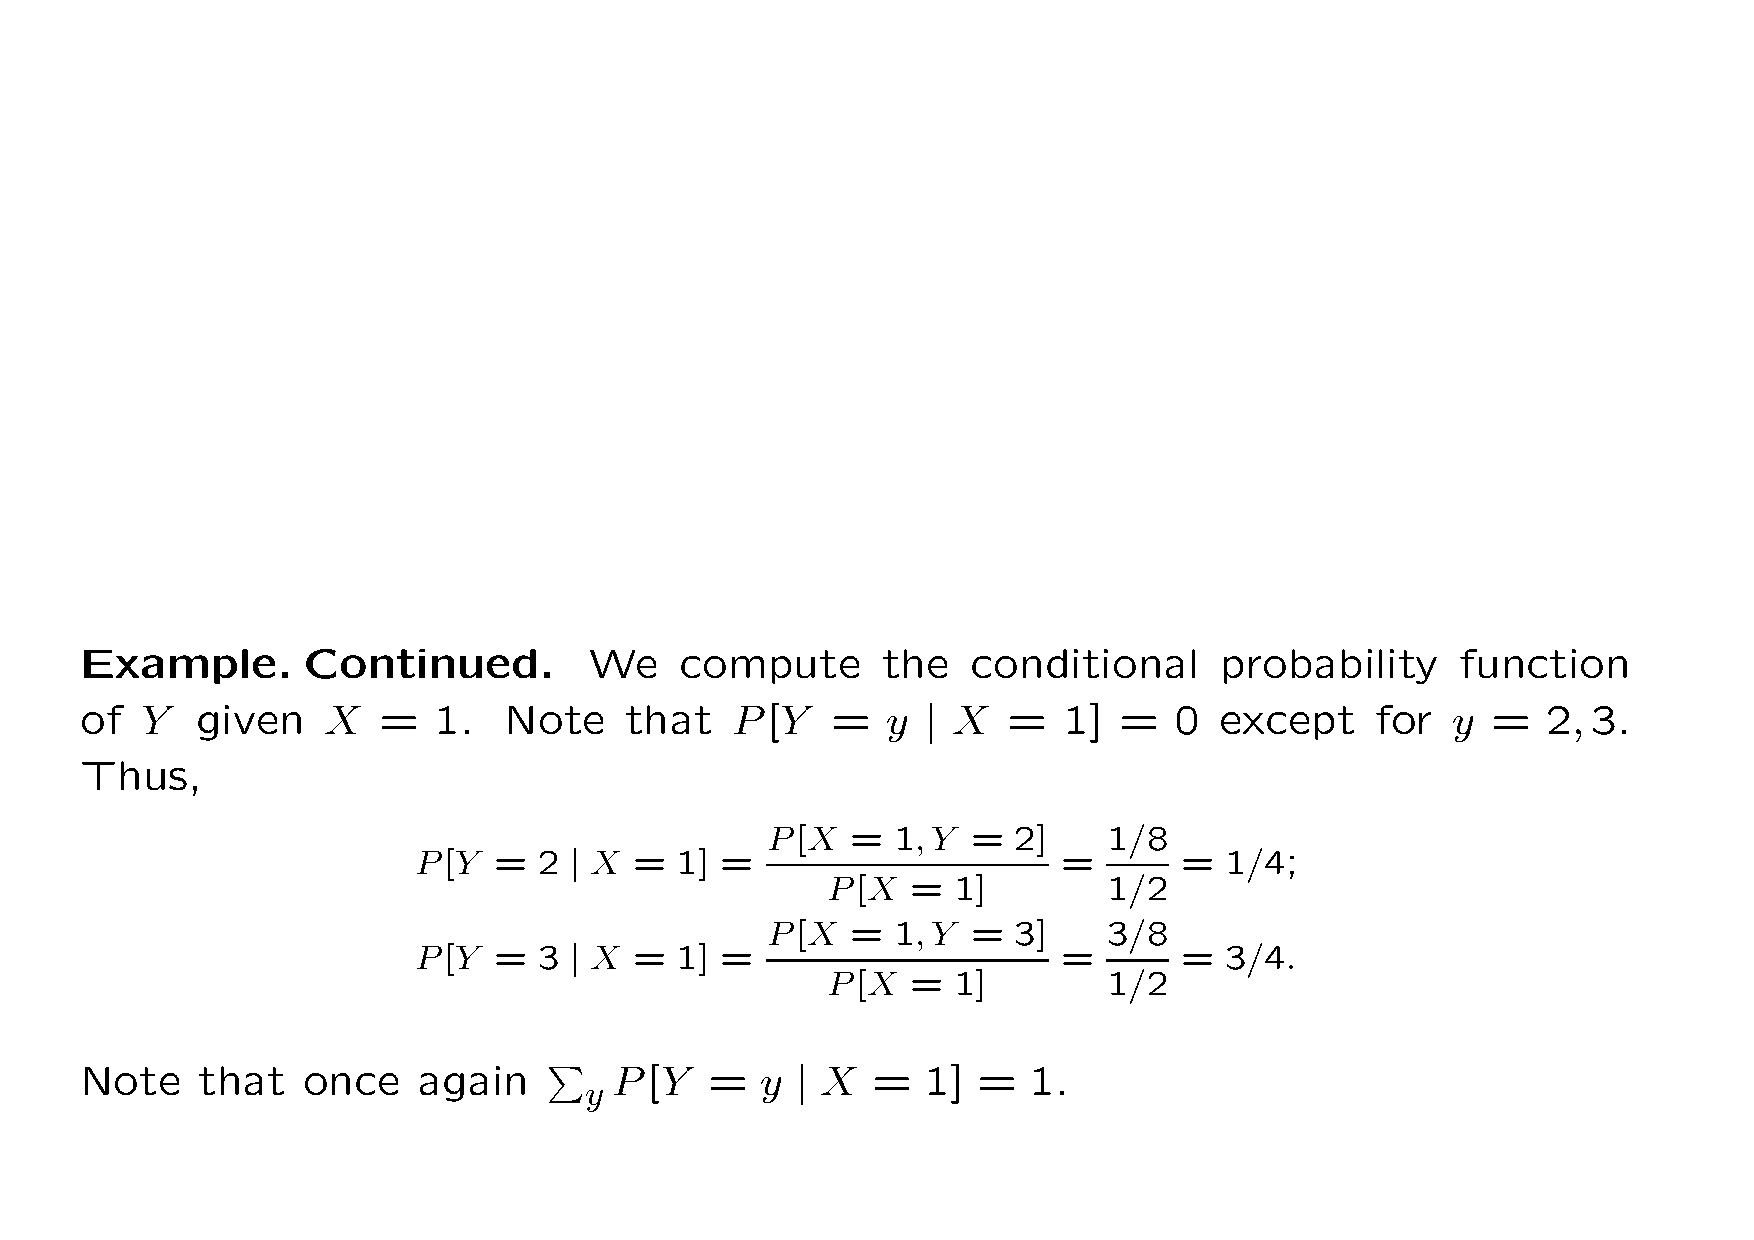
\includegraphics[width=0.9\textwidth,height=0.45\textheight]{ex_audrins_2.pdf}
\end{figure}
\end{example}
\end{frame}


\begin{frame}%
%EndExpansion

\frametitle{Expectations for Jointly Distributed Discrete RVs}

\begin{definition}
Let $h(x,y)$ be a function of $x$ and $y$. 
We define the \textbf{expected value} of $h\left( X,Y\right) $ as%
\begin{equation*}
E\left[ h\left( X,Y\right) \right] =\sum_{y}\sum_{x}h\left( x,y\right)
p_{X,Y}\left( x,y\right)
\end{equation*}
\end{definition}
\end{frame}%




\begin{frame}
\frametitle{Expectations for Jointly Distributed Discrete RVs}
\begin{example}
\begin{figure}[ptb]\centering
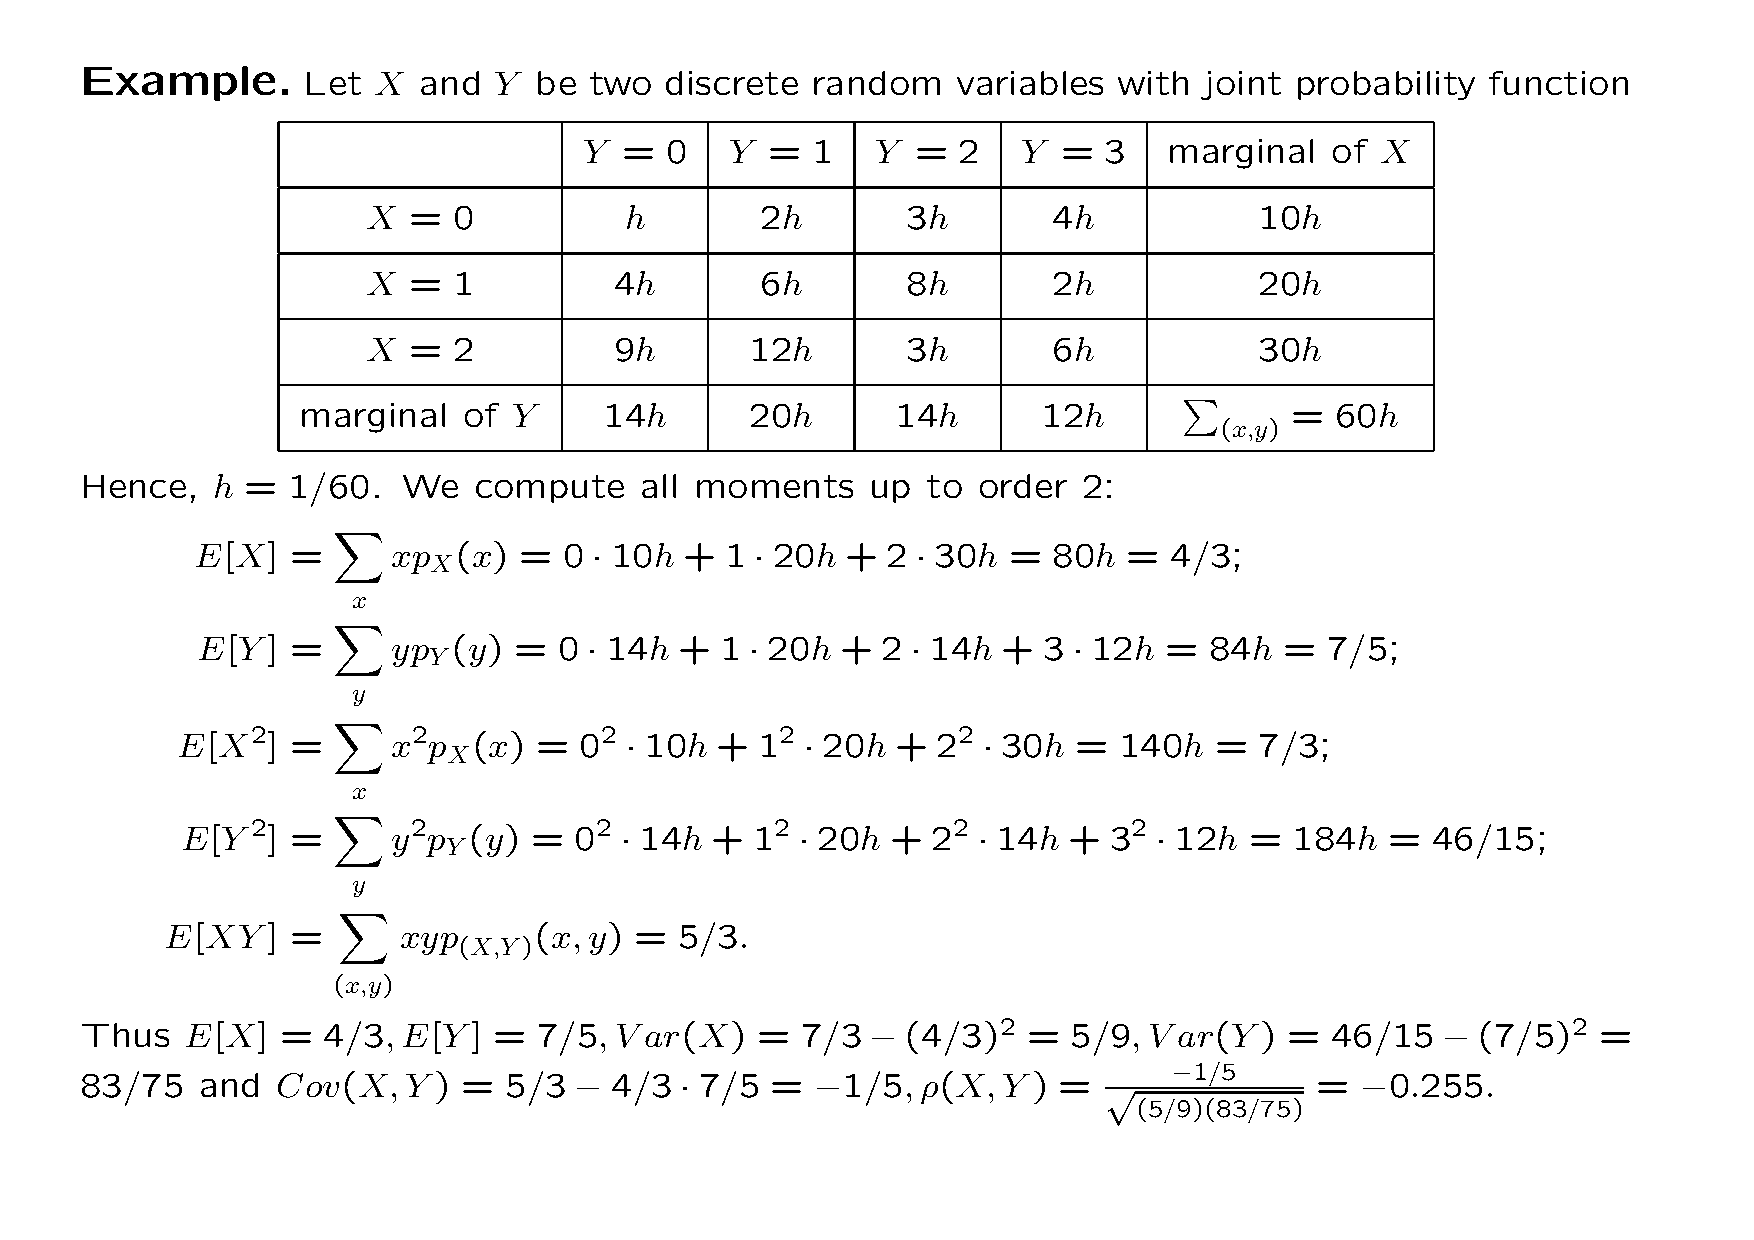
\includegraphics[width=0.85\textwidth,height=0.78\textheight]{ex_tot.pdf}
\end{figure}
\end{example}
\end{frame}

\begin{frame}%
%EndExpansion

\frametitle{Expectations for Jointly Distributed Discrete RVs}

\begin{definition}
The \textbf{conditional expectation }of $h\left( X,Y\right) $ 
\emph{given} $Y=y$ is defined as%
\begin{equation*}
E\left[ h\left( X,Y\right) |y\right] =\sum_{x}h\left( x,y\right)
p_{X|Y}\left( x|y\right).
\end{equation*}

The \textbf{conditional expectation }of $h\left( X,Y\right) $ 
\emph{given} $X=x$ is defined as%
\begin{equation*}
E\left[ h\left( X,Y\right) |x\right] =\sum_{y}h\left( x,y\right)
p_{Y|X}\left( y|x\right).
\end{equation*}
\end{definition}

%TCIMACRO{\TeXButton{EndFrame}{\end{frame}}}%
%BeginExpansion
\end{frame}%



\begin{frame}
\frametitle{Expectations for Jointly Distributed Discrete RVs}
\begin{example}[continuing the example at page 10]
\begin{figure}[ptb]\centering
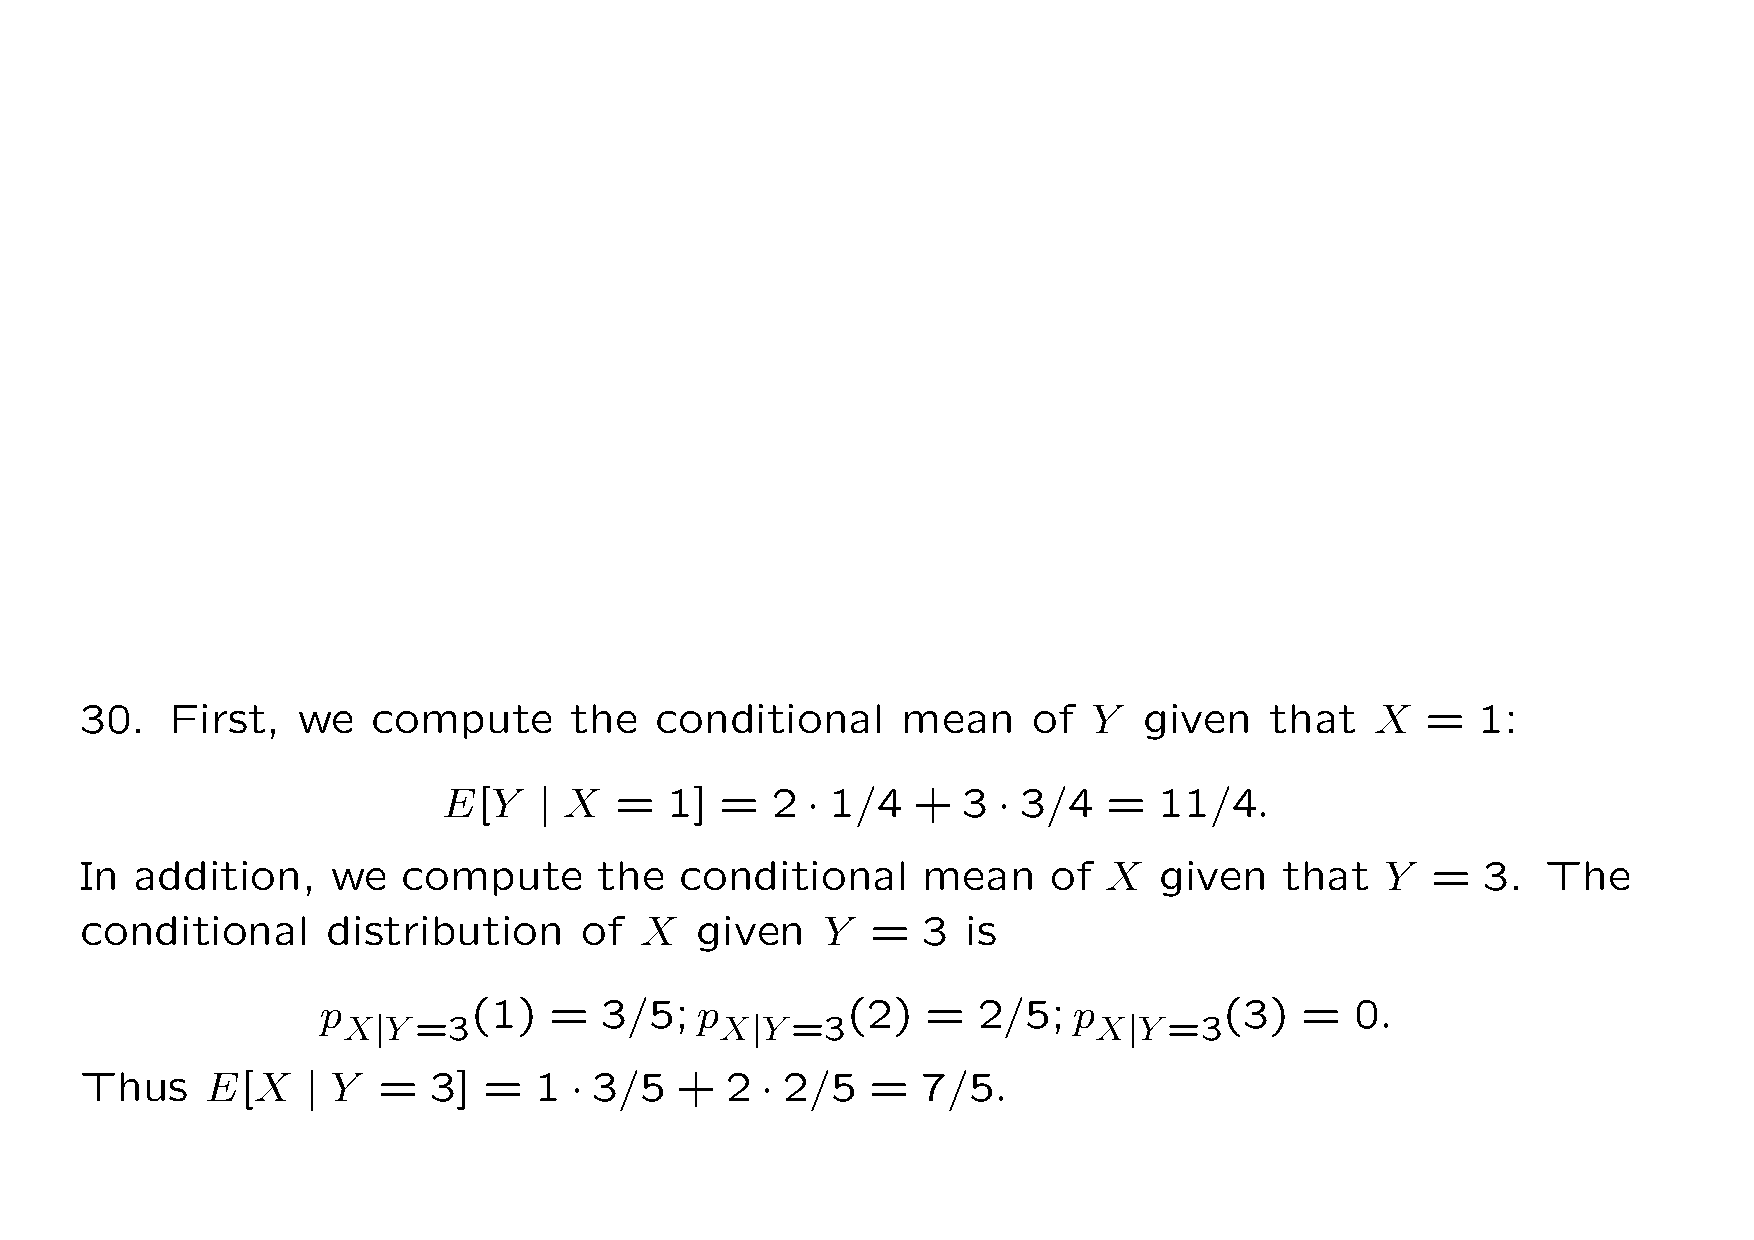
\includegraphics[width=0.9\textwidth,height=0.4\textheight]{ex_cond_audrins.pdf}
\end{figure}
\end{example}
\end{frame}

%EndExpansion
%
%%TCIMACRO{\TeXButton{BeginFrame}{\begin{frame}}}%
%%BeginExpansion
%\begin{frame}%
%%EndExpansion
%
%\frametitle{Expectations for Jointly Distributed Continuous RVs}
%
%\begin{stepitemize}
%\item Let $h(x,y)$ be a function of $x$ and $y$
%
%\item We define the \textbf{expected value} of $h\left( X,Y\right) $ as%
%\begin{equation*}
%E\left[ h\left( X,Y\right) \right] =\int_{y}\int_{x}h\left( x,y\right)
%f_{X,Y}\left( x,y\right) dxdy
%\end{equation*}
%
%\item Further, the \textbf{conditional expectation }of $h\left( X,Y\right) $ 
%\emph{given} $Y=y$ is defined as%
%\begin{equation*}
%E\left[ h\left( X,Y\right) |Y=y\right] =\int_{x}h\left( x,y\right)
%f_{X|Y}\left( x|y\right) dx
%\end{equation*}
%
%\item And, the \textbf{conditional expectation }of $h\left( X,Y\right) $ 
%\emph{given} $X=x$ is defined as%
%\begin{equation*}
%E\left[ h\left( X,Y\right) |X=x\right] =\int_{y}h\left( x,y\right)
%f_{Y|X}\left( y|x\right) dy
%\end{equation*}
%\end{stepitemize}
%
%%TCIMACRO{\TeXButton{EndFrame}{\end{frame}}}%
%%BeginExpansion
%\end{frame}%
%%EndExpansion
%
%%TCIMACRO{\TeXButton{EndFrame}{\end{frame}}}%
%%BeginExpansion
%\end{frame}%
%%EndExpansion
%

\begin{frame}%

\frametitle{Iterated Expectations}

\begin{definition}
The \textit{law of the iterated expectation} is often stated in the
form 
\begin{equation*}
E[h(X,Y)]=E[E[h(X,Y)|Y]]=E[E[h(X,Y)|X]]\,. 
\end{equation*}
\end{definition}

\begin{stepitemize}

\item This notation emphasises that whenever we write down $E[\cdot]$ for an
expectation we are taking that expectation with respect to the distribution
implicit in the formulation of the argument. 

\item The above formula is perhaps more easily understood using the more
explicit notation  
\begin{equation*}
E_{(X,Y)}[h(X,Y)]=E_{(Y)}[E_{(X|Y)}[h(X,Y)]]=E_{(X)}[E_{(Y|X)}[h(X,Y)]]\,. 
\end{equation*}

\item The latter notation makes it clear what distribution is being used to
evaluate the expectation, the joint, the marginal or the conditional.
\end{stepitemize}

%TCIMACRO{\TeXButton{EndFrame}{\end{frame}}}%
%BeginExpansion
\end{frame}%




\begin{frame}
\frametitle{Expectations for Jointly Distributed Discrete RVs}

\begin{definition}
Let $X$ and $Y$ be two discrete random variables. 
The \textbf{covariance} between $X$ and\textbf{\ }$Y$ is given by $%
E\left[ h\left(X,Y\right) \right] $ when%
\begin{equation*}
h\left(X,Y\right) =%
\left(X-E\left[ X\right] \right) \left( Y-E\left[ Y\right] \right),%
\end{equation*}
i.e. $Cov\left(X,Y\right) =E\left[ \left(X-E\left[ X\right] \right)
\left(Y-E\left[ Y\right] \right) \right] $
\end{definition}

Alternative formula\footnote{To get it, expand 
$$\left(X-E\left[ X\right] \right) \left( Y-E\left[ Y\right] \right)=XY-E\left[ X\right]Y -XE\left[ Y\right] +E\left[ X\right]E\left[ Y\right]$$ and make use of the properties of expectation.} for $Cov(X,Y)$ is%
\begin{equation}
\boxed{Cov\left( X,Y\right) =E\left[ XY\right] -E\left[ X\right] E\left[ Y\right]\ .} \label{Cov}
\end{equation}

\end{frame}


\begin{frame}
\frametitle{Expectations for Jointly Distributed Discrete RVs}

So, to compute the covariance from a table describing the joint behaviour of $X$ and $Y$, you have to:

\begin{itemize}
\item compute the joint expectation $E[XY]$---you get it making use of the joint probability; \vspace{0.2cm}
\item compute $E[X]$ and $E[Y]$---you get using the marginal probability for $X$ and $Y$; \vspace{0.2cm}
\item combine these expected values as in formula (\ref{Cov}). 

\end{itemize}

See example on page 13 for an illustrative computation.

\end{frame}



\begin{frame}%

\frametitle{Some Properties of Covariances }


    \begin{stepitemize}

\item The Cauchy-Schwartz Inequality states 
$$(E\left[ XY\right])^2\leq E\left[ X^2\right]E\left[ Y^2\right],
$$ 
with equality if, and only if, $\Pr(Y=cX)=1$ for some constant $c$.

\vspace{0.4cm}

\item Let $h(a)=E[(Y-aX)^2]$ where $a$ is any number. Then
$$
0\leq h(a)=E[(Y-aX)^2]=E[X^2]a^2-2E[XY]a+E[Y^2]\,.
$$
This is a quadratic in $a$, and
\item[-] if $h(a)>0$ the roots are real and $4(E[XY])^2-4E[X^2]E[Y^2]<0$,
\item[-] if $h(a)=0$ for some $a=c$ then $E[(Y-cX)^2]=0$, which implies that $\Pr(Y-cX=0)=1$.
\end{stepitemize}
\end{frame}%


\begin{frame}%
%EndExpansion

\frametitle{Some Properties of Covariances}
\begin{small}
\begin{remark} 
 If two random variables are independent, their covariance is equal to
zero. Note that the converse is not necessarily true: a zero covariance
between two random variables does not imply that the variables are 
independent. This asymmetry\footnote{Independence $\Rightarrow Cov(X,Y)=0$ but $Cov(X,Y)=0\nRightarrow$ independence.} follows because \textbf{the covariance is  a `measure' of linear dependence.}
\end{remark}
\begin{example}

Let us consider two discrete random variable $X$ and $Y$, such that
$$
P(\{X=0\})=P(\{X=1\})=P(\{X=-1\})=\frac{1}{3},
$$
while $Y=0$ if $X\neq 0$ and $Y=1$, if $X=0$. So we have $E[X]=0$ and $XY=0$. This implies
$$
Cov(X,Y) = E[XY] -E[X]E[Y] =0,
$$ 
although $X$ and $Y$ are NOT independent: they are related in a nonlinear way. 

\end{example}
\end{small}

\end{frame}

\begin{frame}%
%EndExpansion

\frametitle{Some Properties of Covariances}

Building on this remark, we have

\begin{stepitemize}

\item 
%TCIMACRO{\TeXButton{black}{\color{black}}}%
%BeginExpansion
\color{black}%
%EndExpansion
$Cov(X,Y)>0$ if
\begin{stepitemize}
\item large values of $X$ tend to be \emph{linearly }associated with large
values of $Y$
\item small values of $X$ tend to be \emph{linearly }associated with small
values of $Y$\bigskip
\end{stepitemize}
\item $Cov(X,Y)<0$ if
\begin{stepitemize}
\item large values of $X$ tend to be \emph{linearly }associated with
\underline{small} values of $Y$
\item small values of $X$ tend to be \emph{linearly }associated with
\underline{large} values of $Y$\bigskip
\end{stepitemize}
\item When $Cov(X,Y)=0$, $X$ and $Y$ are said to be uncorrelated.
\end{stepitemize}
%
%\textbf{GIACOMO DIMOSTRA PROP 4.2 del Ross a tutorial}
\end{frame}
%
\begin{frame}%
%%EndExpansion
%
\frametitle{Some Properties of Covariances}
%
\begin{stepitemize}
\item  If $X$ and $Y$ are two random variables (either discrete or continuous) with $Cov(X,Y) \neq 0$, then:
\begin{equation}
Var(X + Y) =  Var(X) + Var(Y) + 2 Cov(X,Y) \label{FullVar}
\end{equation}

\underline{Compare this expression with the formula on page 25, Lecture 3-4}, where we read that in the case of independent random variables $X$ and $Y$
we have
$$
Var(X + Y) =  Var(X) + Var(Y),
$$
which trivially follows from (\ref{FullVar})---indeed, for independent random variables, $Cov(X,Y)\equiv 0$.

\item The covariance depends upon the unit of measurement.


\end{stepitemize}
%
\end{frame}


\begin{frame}
\frametitle{A remark}

\begin{stepitemize}
\item If we scale $X$ and $Y$, the covariance changes: For $a,b>0$%
\begin{equation*}
Cov\left( aX,bY\right) =abCov\left( X,Y\right)
\end{equation*}

Thus, we introduce the\textbf{\ correlation} between $X$ and $Y$ is
\begin{equation*}
corr\left( X,Y\right) =\frac{Cov\left( X,Y\right) }{\sqrt{Var\left( X\right)
Var\left( Y\right) }}
\end{equation*}

which \emph{does not }depend upon the unit of measurement.


\end{stepitemize}


\end{frame}


%
%\begin{stepitemize}
%\item Proof: For $a,b>0$%
%\begin{eqnarray*}
%corr\left( aX,bY\right)  &=&%
%%TCIMACRO{\TeXButton{Pause}{\pause}}%
%%BeginExpansion
%\pause%
%%EndExpansion
%\frac{Cov\left( aX,bY\right) }{\sqrt{Var\left( aX\right) Var\left( bY\right)
%}}\medskip
%%TCIMACRO{\TeXButton{Pause}{\pause} }%
%%BeginExpansion
%\pause
%%EndExpansion
%\\
%&=&\frac{abCov\left( X,Y\right) }{\sqrt{a^{2}Var\left( X\right)
%b^{2}Var\left( Y\right) }}\medskip
%%TCIMACRO{\TeXButton{Pause}{\pause} }%
%%BeginExpansion
%\pause
%%EndExpansion
%\\
%&=&\frac{abCov\left( X,Y\right) }{ab\sqrt{Var\left( X\right) Var\left(
%Y\right) }}\medskip
%%TCIMACRO{\TeXButton{Pause}{\pause} }%
%%BeginExpansion
%\pause
%%EndExpansion
%\\
%&=&Corr\left( X,Y\right) \medskip
%%TCIMACRO{\TeXButton{Pause}{\pause}}%
%%BeginExpansion
%\pause%
%%EndExpansion
%\end{eqnarray*}
%\end{stepitemize}


\begin{frame}%
%%EndExpansion
%
\frametitle{An important property of correlation}
\begin{remark}
The Cauchy-Schwartz Inequality implies that 
%Applying the Cauchy-Schwartz Inequality to $U=X-E\left[ X\right]$ and $V=Y-E\left[ Y\right]$ indicates that%
\begin{equation*}
-1\leq corr\left( X,Y\right) \leq 1
\end{equation*}
\end{remark}

\vspace{0.4cm}

The correlation is typically denoted by the Greek letter $\rho$, so we have 
$$
\rho(X,Y)= corr\left( X,Y\right).
$$
\end{frame}%


\end{document}
